\newcommand{\optResults}{\begin{table}[H]\centering\small
\begin{tabular}{lccccccccc}\toprule
 & $z$ & $V/\bar\lambda$ & $\varepsilon$ & $\alpha_D$ & $\alpha_S$ & $\alpha_\lambda$ & $s_S$ & $s_\lambda$ & \textbf{Real score}\\\midrule
starting point & 0.50 & 1.00 & 0.020 & 1.00 & 0.00 & 0.00 & 1.00 & 1.00 & 18.26\\
\textbf{potential optimum} & 0.42 & 1.11 & 0.018 & 1.00 & 0.00 & 0.04 & 0.96 & 0.93 & 18.30\\
perfect information (control) & 0.61 & 0.78 & 0.016 & 0.85 & 0.00 & 0.00 & 0.95 & 0.73 & 19.67\\
\bottomrule\end{tabular}
\caption{Coefficients before and after optimising the potential (23 local Nelder--Mead runs in 4 workers;
688 scenario-set evaluations). ``Real score'': the 12 concatenated pseudo-test weeks. The last row is the
perfect-information case: the ceiling of the controller, with the global oracle at 19.92.}
\end{table}
\begin{figure}[H]\centering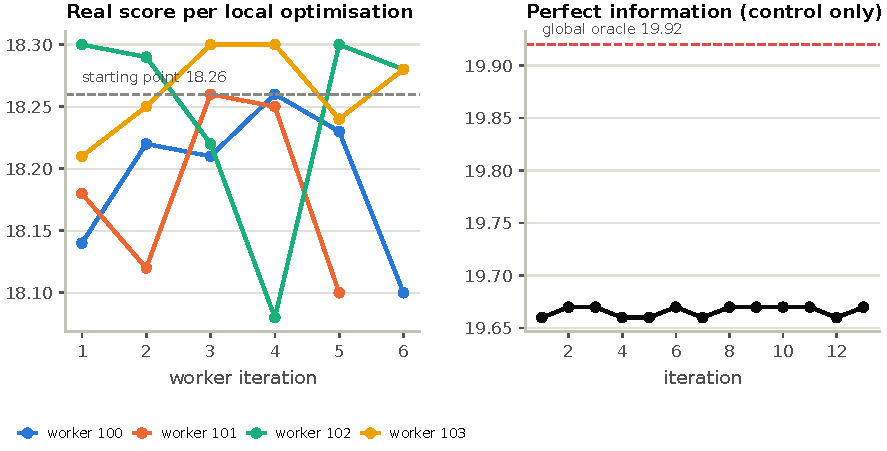
\includegraphics[width=\linewidth]{fig/potential.pdf}
\caption{Left: real score reached by each worker after each local optimisation (the shared record only goes up). Right: the perfect-information worker.}\end{figure}
}
